
\chapter{Design and Implementation}
\label{design}
In this chapter we present a brief overview of the library
by explaining its overall structure and how to extend it.

\subsection*{Dependencies}
To run recsyslab, one needs a Python 2.7.x interpreter~\cite{python} and NumPy~\cite{numpy},
a package for scientific computing with Python, to be installed.

\subsection*{Input Dataset Format}
At the moment, only one type of dataset is supported. The dataset has to be
a textfile where each line is of this form:

\begin{lstlisting}
UserID<separator>ItemID<separator>NumberOfInteractions
\end{lstlisting}

<separator> is an arbitrary string, but it has to be the same throughout the whole dataset.
NumberOfInteractions is optional and can be omitted. In this case one will be assumed.
Everything that follows NumberOfInteractions<separator> will be ignored.
Please note that when you are omitting NumberOfInteractions but have something else after
the ItemId, this will be recognized as NumberOfInteractions.

We recommend to use the MovieLens database (see \ref{movielens}) with 100,000 ratings.
It is easy to obtain, does not need any modifications to work with our library and has a
reasonable size. Additionaly, we will use this dataset in the examples of the user manual in 
Chapter~\ref{usermanual}.

%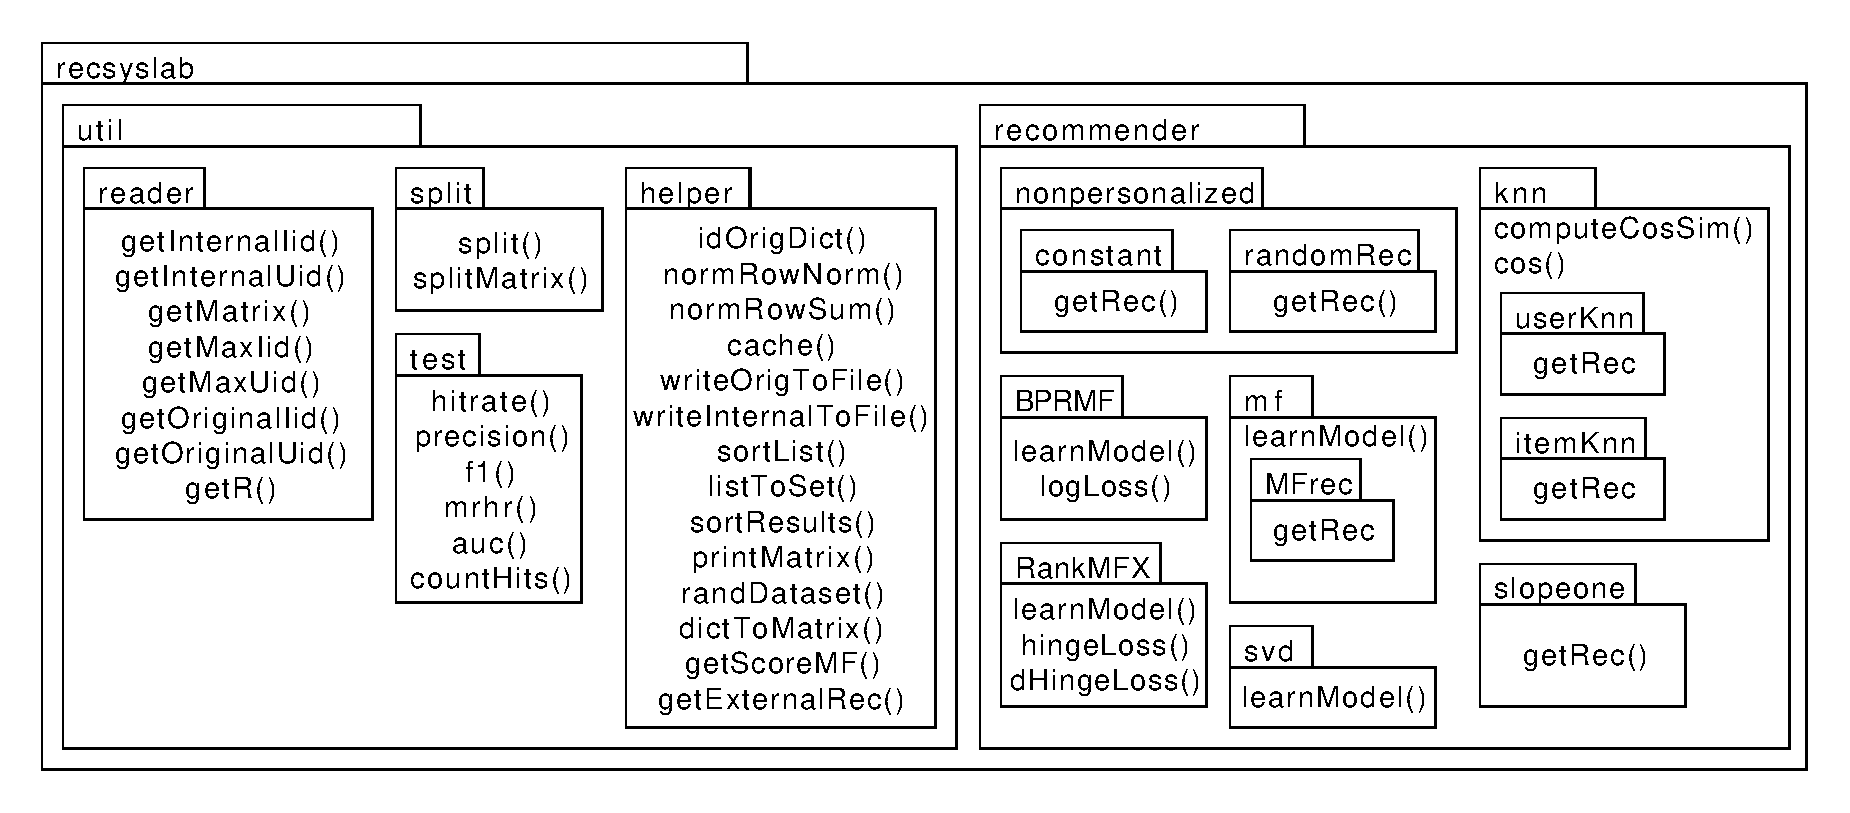
\includepdf[angle=90]{packagediagram.pdf}
\pagebreak
\section{General structure}
Here is a figure illustrating the structure of recsyslab:

\begin{figure}[H]
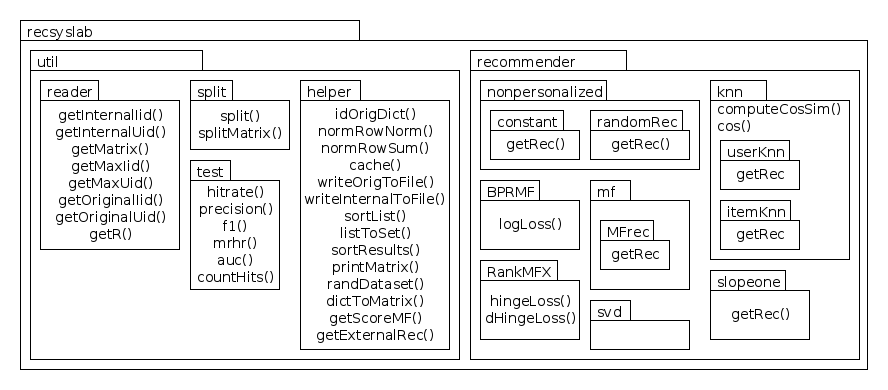
\includegraphics[scale=0.4]{packagediagram.png}
\caption{Structure of recsyslab.}
\end{figure}

\subsection*{The Util Package}
The util package contains several modules for the things happening around the 
recommender algorithms and the methods for the test metrics.
The modules in the util package are:
\begin{description}
\item[reader] manages the data
\item[split] splits up the dataset following the leave-one-out protocol, see also Chapter~\ref{background}
\item[helper] contains several helper functions
\item[test] contains the methods for computing the test metrics
\end{description}
The \lstinline!reader! module is a very central part in recsyslab.
The class \lstinline!reader! in the module reader takes care of reading the dataset and 
supplies the other parts of recsyslab with the kinds of data they need.
While the reader reads the dataset, it maps the UserIDs and 
ItemIDs from the original IDs in the dataset to internal IDs 
starting at zero and counting up. This guarantees that the IDs are consecutive. 
When the IDs are consecutive, it is possible to use them as
indices in a matrix.
Furthermore, the reader constructs a dict and a matrix
out of the data using the internal IDs. The dict has the internal 
UserIDs as keys and the values are tuples representing the 
interactions of the corresponding user. The first value of these tuples is the internal
ItemID of the interaction, the second is the intensity or
quantity of the interaction. You can get the dict by calling \lstinline!getR()!
of the \lstinline!reader! object.
The matrix offered by a reader has as many lines as the dataset
has users and as many columns as the items that are present in the dataset.
The entry at the i-th line and j-th column is then the intensity of the interaction
between user i and item j. A zero means that there has not been any
interaction yet.
The k-Nearest-Neighbor algorithms need a matrix, like it is provided by a
reader. All other recommendation algorithms need a dict of the 
form described above.

\subsection*{The Recommender Package}
The recommender package contains all recommender algorithms.
They are separated into the following modules:
\begin{description}
\item[nonpersonalized] simple, nonpersonalized algorithms
\item[knn] k-Nearest-Neighbors algorithms
\item[mf] Pairwise matrix factorization algorithms
\item[BPRMF] Bayesian Personalized Ranking Matrix Factorization algorithm
\item[RankMFX] RankMFX algorithm
\item[slopeone] Slope One algorithm
\item[svd] Ranking SVD (Sparse SVD)
\end{description}
These modules do not have a \lstinline!learnModel()! method yet, because the model is trained when the object is instantiated.
For descriptions of the algorithms please refer to Chapter~\ref{recommendationalgorithms}.

To implement new recommender algorithms which integrate nicely into the infrastructure,
the only thing one has
to take care of, is to provide a \lstinline!getRec! function which has an 
internal UserID as first the first argument and the number of items to recommend
as the second argument. Additionaly, it should return a list of internal ItemIDs of the
length which has been specified in the second argument.
